\documentclass[english]{article}
\usepackage{amsmath}
\usepackage[letterpaper]{geometry}
\usepackage[table,xcdraw]{xcolor}
\usepackage{graphicx}
\graphicspath{ {images/} }
\geometry{verbose,tmargin=1in,bmargin=1in,lmargin=1in,rmargin=1in}
\newcommand\numberthis{\addtocounter{equation}{1}\tag{\theequation}}

\title{ESE 650 Project 5 report: Path Planning}
\author{Dhruva Kumar}
\date{}

\begin{document}

\maketitle

\section{Introduction}
The present task involves finding the shortest path between two points on a aerial map of the Penn campus. This was done for two modalities: vehicles and pedestrians. Imitation learning, specifically an exponentiated functional gradient descent algorithm (LEARCH \cite{c1}) was used to learn the cost map given the tranining paths drawn by an expert. LEARCH tries to imitate the experty policy and updates the cost map iteratively such that the planned path becomes closer to the desired expert path. Loss augmentation is incorporated for getting better and generalized results during testing. This is in line with the philosophy of learning on difficult problems so that problems (testing) becomes simpler. Support Vector Regression (SVR) was used to classify the features for the planned and desired path and the weights were used to update the log cost map. The results for both the modes were found to be pretty good. 

\section{Feature extraction}
The 23 MB original aerial image was rescaled by a factor of 0.2 and binary features were extracted in the HSV color space. k-means was tried but it was found to give better features with manual thresholding. HSV was chosen since it had a broader range in the color space compared to LAB and YCbCr for the image in subject. \\
Post processing was done on the binary feature masks obtained using MATLAB built in morphological operators like bwareopen and imdilate. Permutation and combination of masks were applied to get the following resultant masks:
\begin{enumerate}
\item Road
\item Vegetation
\item Buildings
\item Road + bridge
\end{enumerate}

\begin{figure}[thpb]
\centering
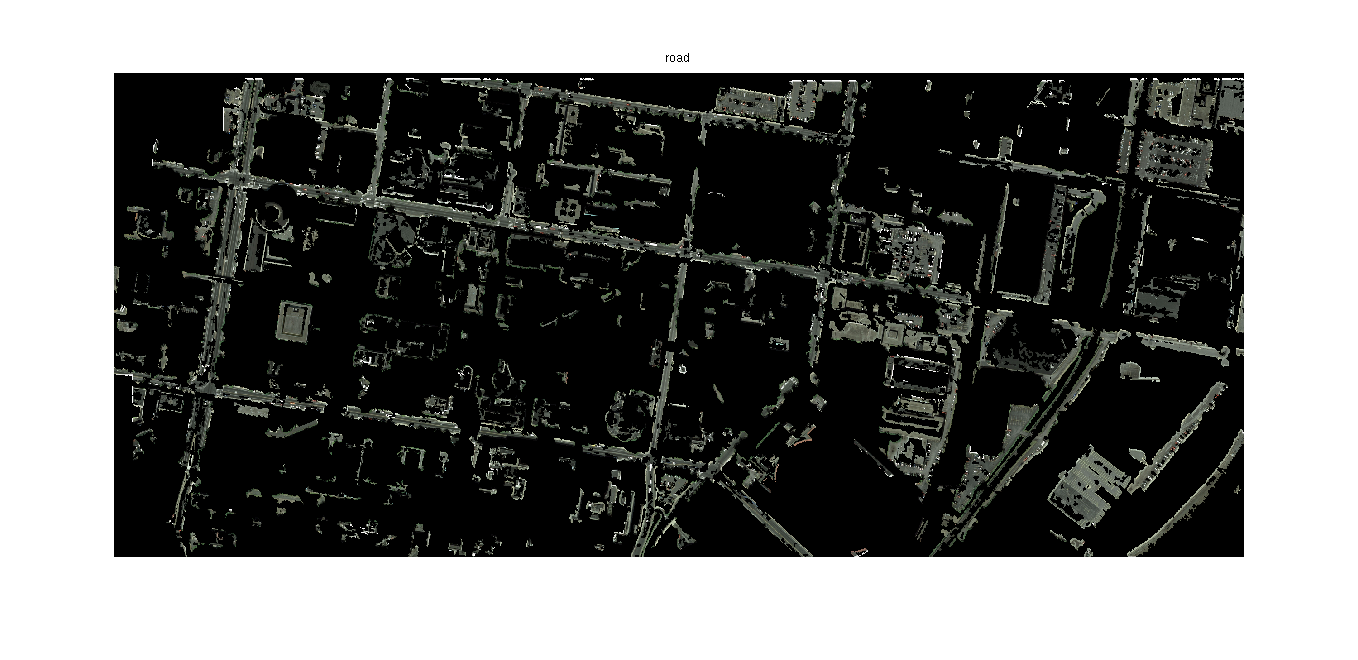
\includegraphics[width=\textwidth]{road}
\caption{Road RGB mask}
\end{figure}

\begin{figure}[thpb]
\centering
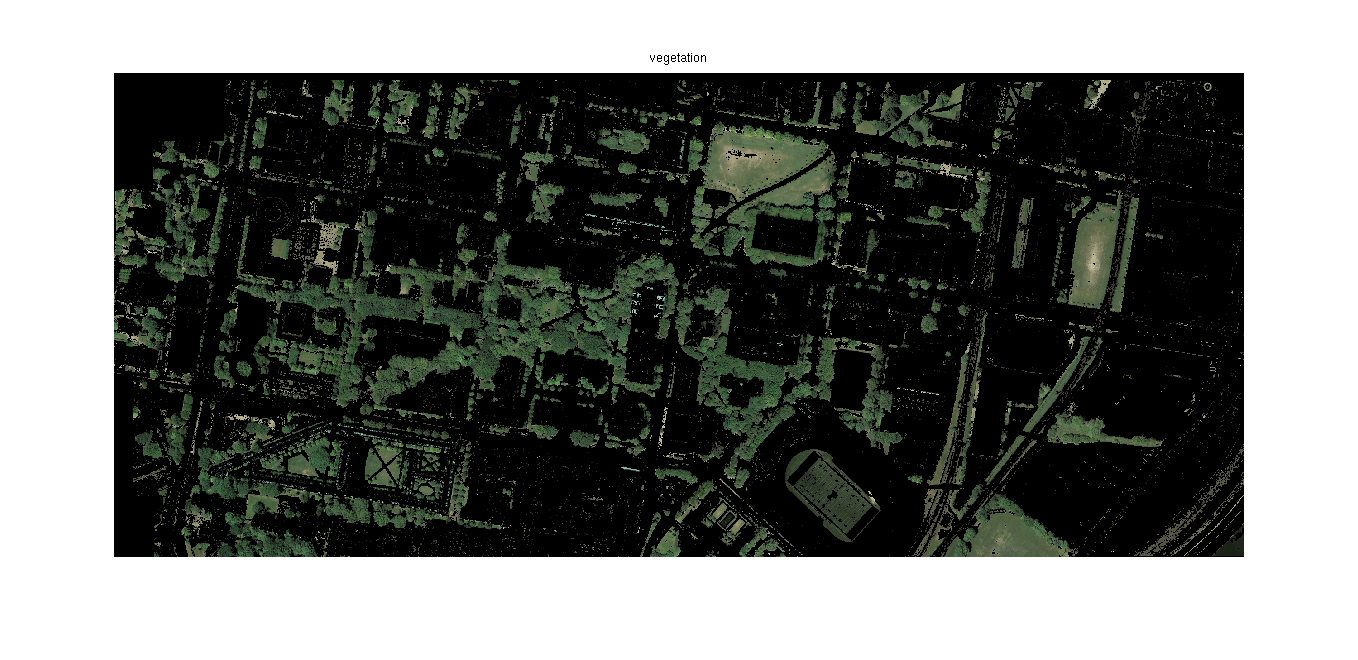
\includegraphics[width=\textwidth]{vegetation}
\caption{Vegetation RGB mask}
\end{figure}

\begin{figure}[thpb]
\centering
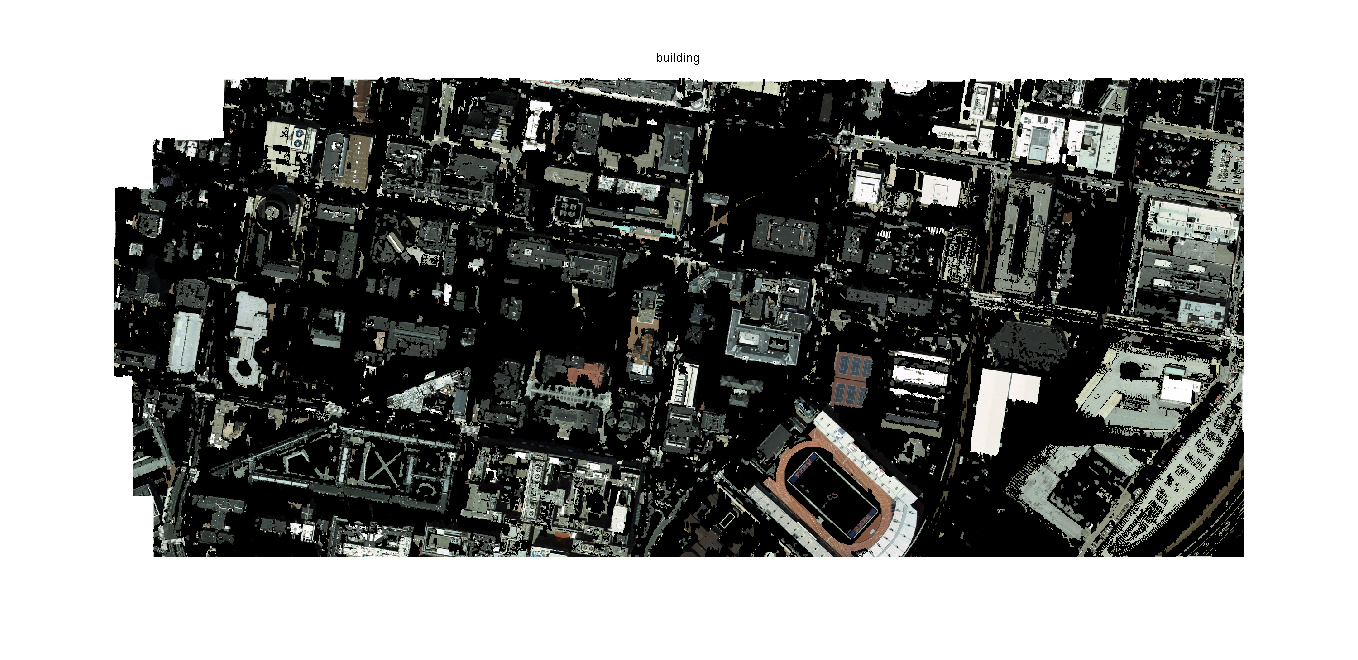
\includegraphics[width=\textwidth]{building}
\caption{Building RGB mask}
\end{figure}

\begin{figure}[thpb]
\centering
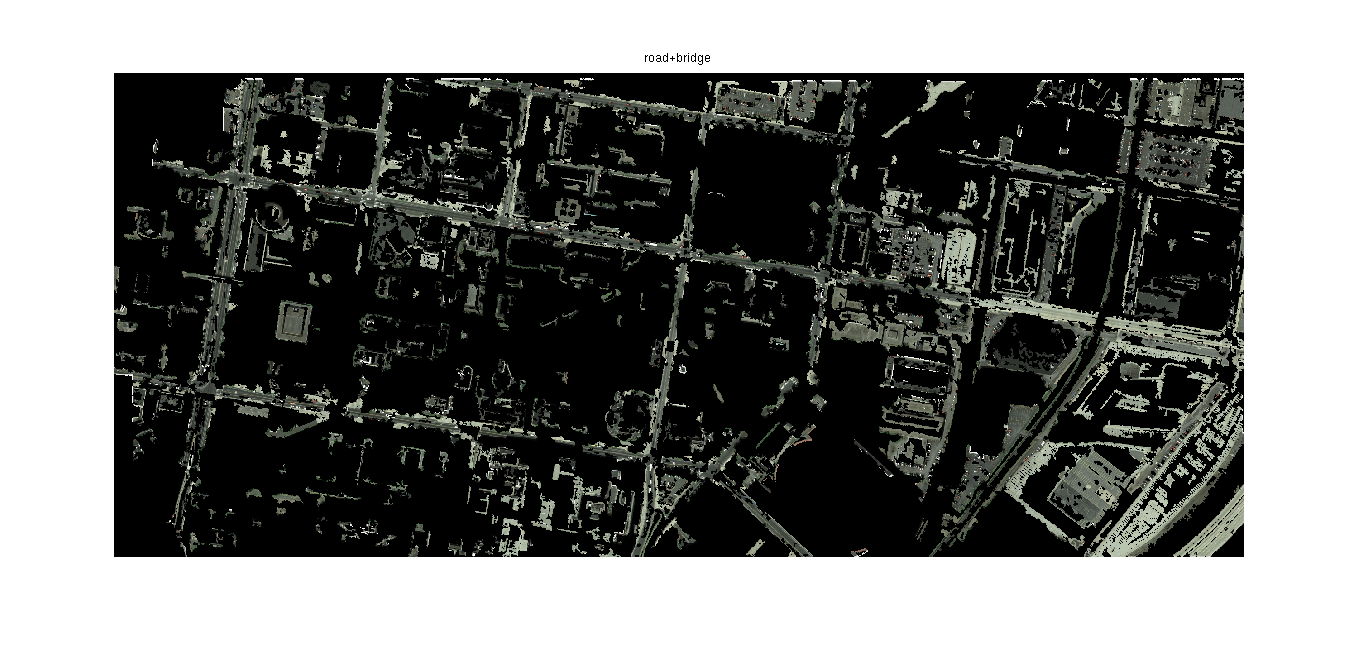
\includegraphics[width=\textwidth]{road+bridge}
\caption{Road + bridge RGB mask}
\end{figure}


\section{LEARCH: LEArning to seaRCH}
The LEARCH algorithm as stated in \cite{c1} (algorithm 5) was implemented with a few changes: \\
\begin{itemize}
\item Training was done for both the modalities: vehicle and pedestrians. 7 paths were manually plotted according to the desired modality and the loss function for each was also computed. The negative examples were precomputed before training. 

\item Dijkstra's algorithm was used to find the shortest planned path given the loss augmented cost map

\item L2-regularized L2-loss support vector regression (SVR) from the liblinear package \cite{c2} was used to classify the positive (planned path) and negative examples (desired path). While updating the log costmap, the weights procured from the SVR were scaled and used to update instead of rounding them off to -1 or +1.
\begin{center}
$s_{t+1} = s_{t} + \alpha_t h_t$ 
\end{center}
Here, $h_t$ is the predicted weight from SVR rescaled between -1 to 1 

\item After the first iteration it was found out that the loss augmented cost map might have potential negative values which would affect Dikjstra. Therefore, the values were scaled to the positive domain. 

\item The 7 training exmples were executed for 150 iterations with the learning rate $\alpha$ = 0.1 for both the modalities. 

\end{itemize}

\paragraph{Loss function: generalization of the hamming window}
A generalization of the hamming window as described in the paper was used. A custom function was created for this purpose. A 1-D hamming window is given by :

\begin{align*}
w(n) = 0.54 - 0.46 \cos (2\pi \frac{n}{N}) \ 0 \leq n \leq N \numberthis
\end{align*}

where the window length $L = N + 1$ \\
This was generalized to 2-D and was shifted and plotted along the desired path according to the expert policy. A hamming window loss function looks like:

\begin{figure}[thpb]
\centering
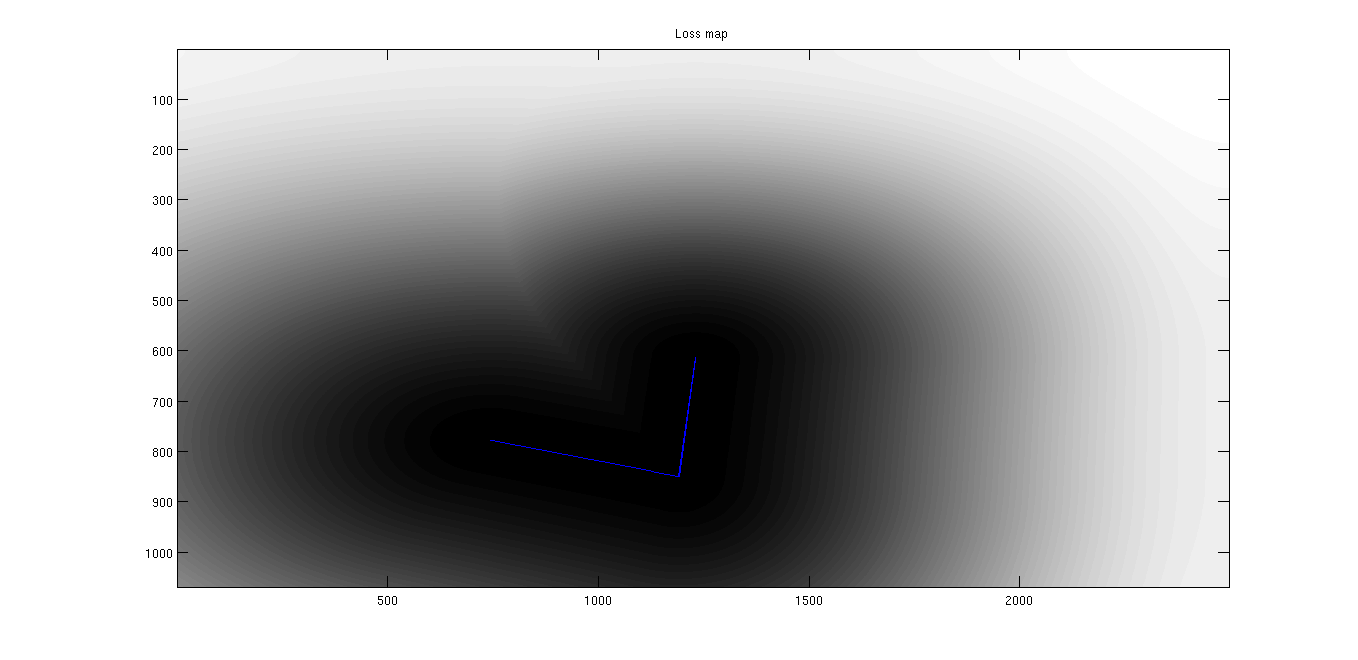
\includegraphics[width=\textwidth]{lossMap}
\caption{Generalized 2-D Hamming window loss function for the desired path (in blue). It's 0 near the path and gradually spreads towards 1 as given in (1)}
\end{figure}

\section{Results}
The results for the road modality were pretty good. The bridge wasn't identified as a part of the road feature initially as a result of which this feature was explcitly added and training paths were given for the LEARCH algorithm to learn this as a part of the road. The problem of the shadowed road between 35 and 34 spruce not being identified  was fixed by choosing better features and giving trained path along this route. A few problems faced was the path plotted being through the parking lot instead of the road. This was due to the color of the parking lot and the road being similar. Another problem was the road in front of the franklin field. Due to it being covered by trees, the minimum cost path was around it, through the building. A fix would be to give training paths in such a manner that buildings would be of a much higher cost than the vegetation. Apart from these two problems, given any two points, it pretty much follows the road. \\
The pedestrian modality also works pretty well except for sometimes flying across the upper buildings as if it were spiderman. A hacky solution would be to lower the cost of the road (after learning). At present, the cost of the roads are low in comparison to the buildings but making it even lower in magnitude will have the result of it traversing only through roads. This was tried and tested and it worked well. But it felt like I was overfitting a tad too much and left the idea. \\

\textbf{Please note: } Some results are posted here. Further results are present in the 'results' directory. 


\begin{figure}[thpb]
\centering
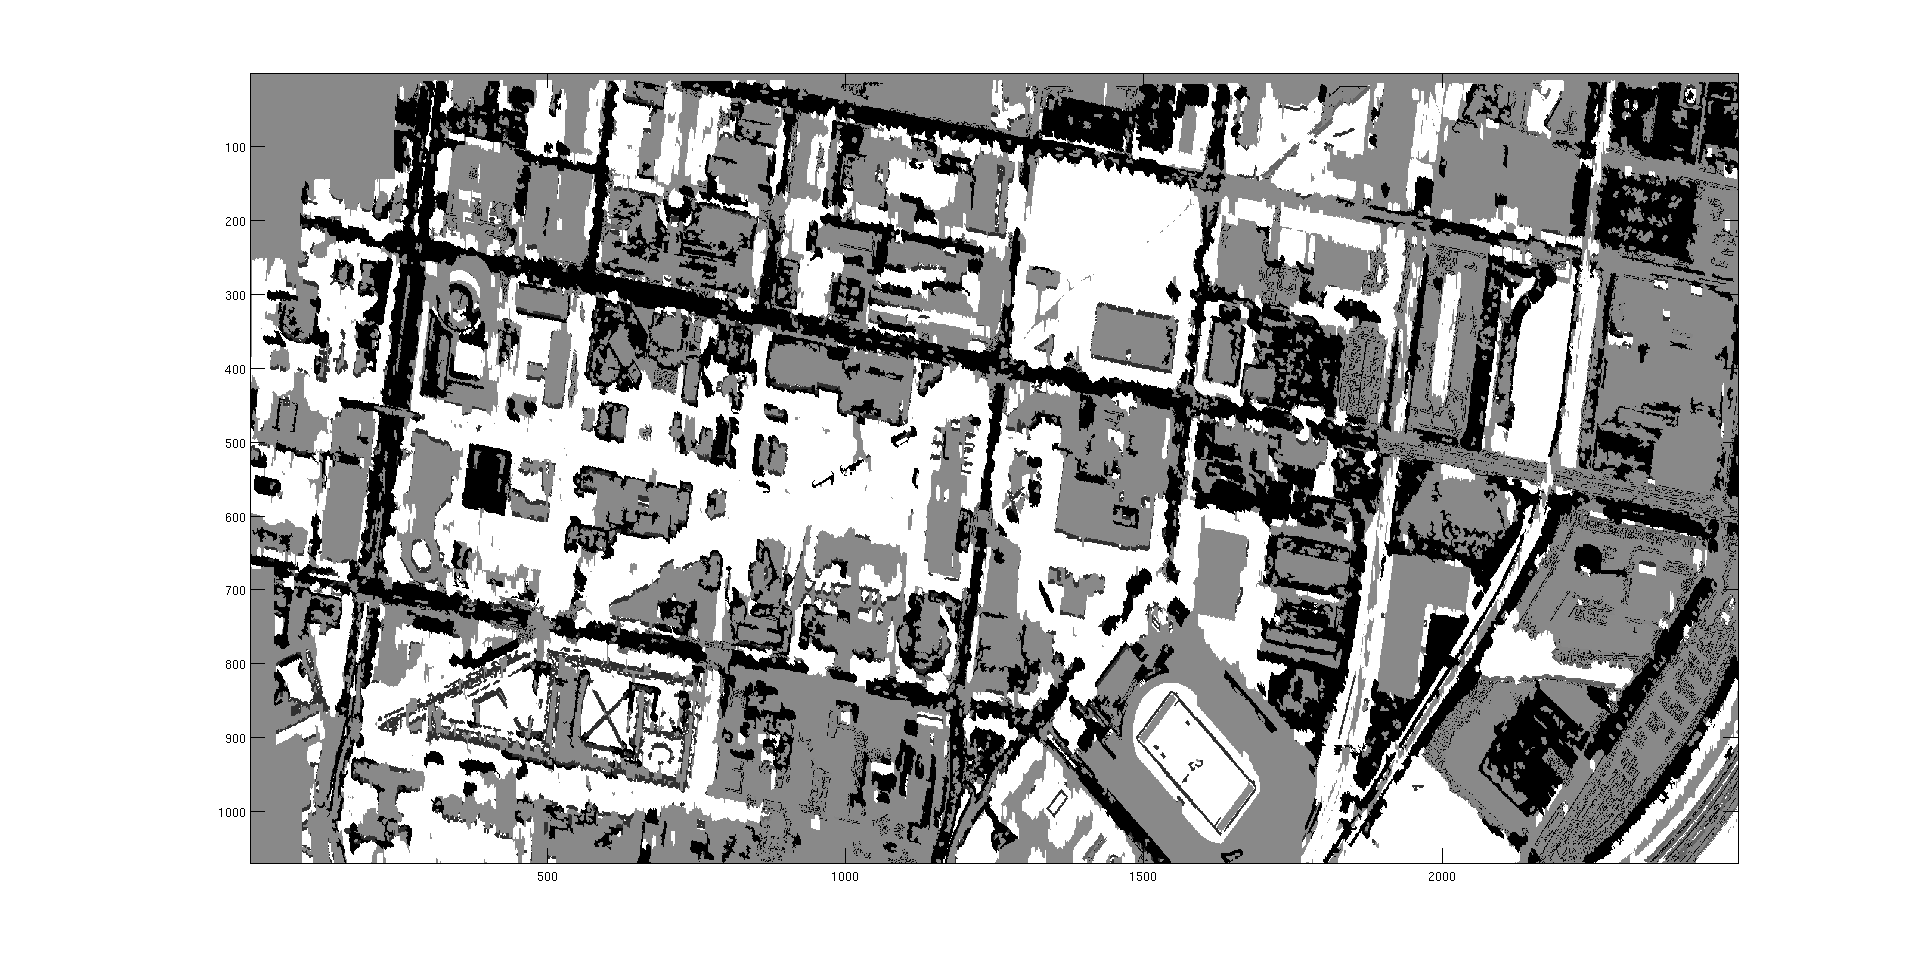
\includegraphics[width=\textwidth]{costMapVeh}
\caption{Cost map for the vehicle mode after learning}
\end{figure}

\begin{figure}[thpb]
\centering
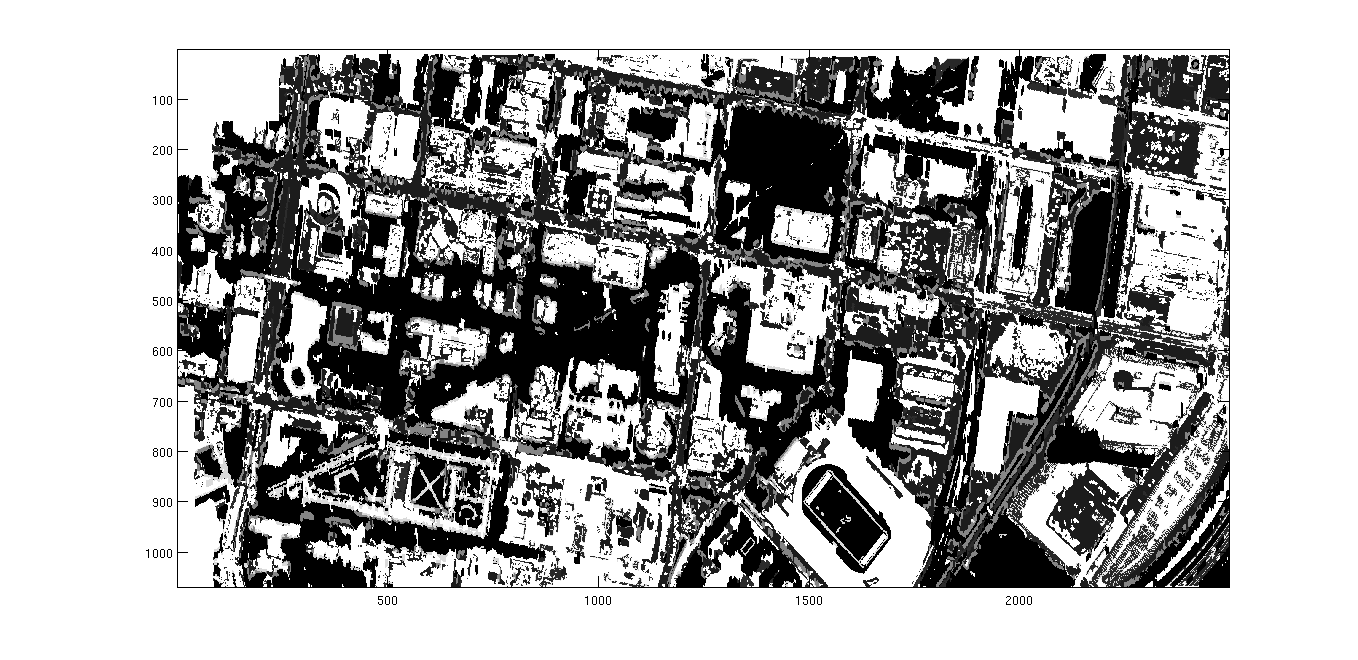
\includegraphics[width=\textwidth]{costMapPed}
\caption{Cost map for the pedestrian mode after learning}
\end{figure}

\begin{figure}[thpb]
\centering
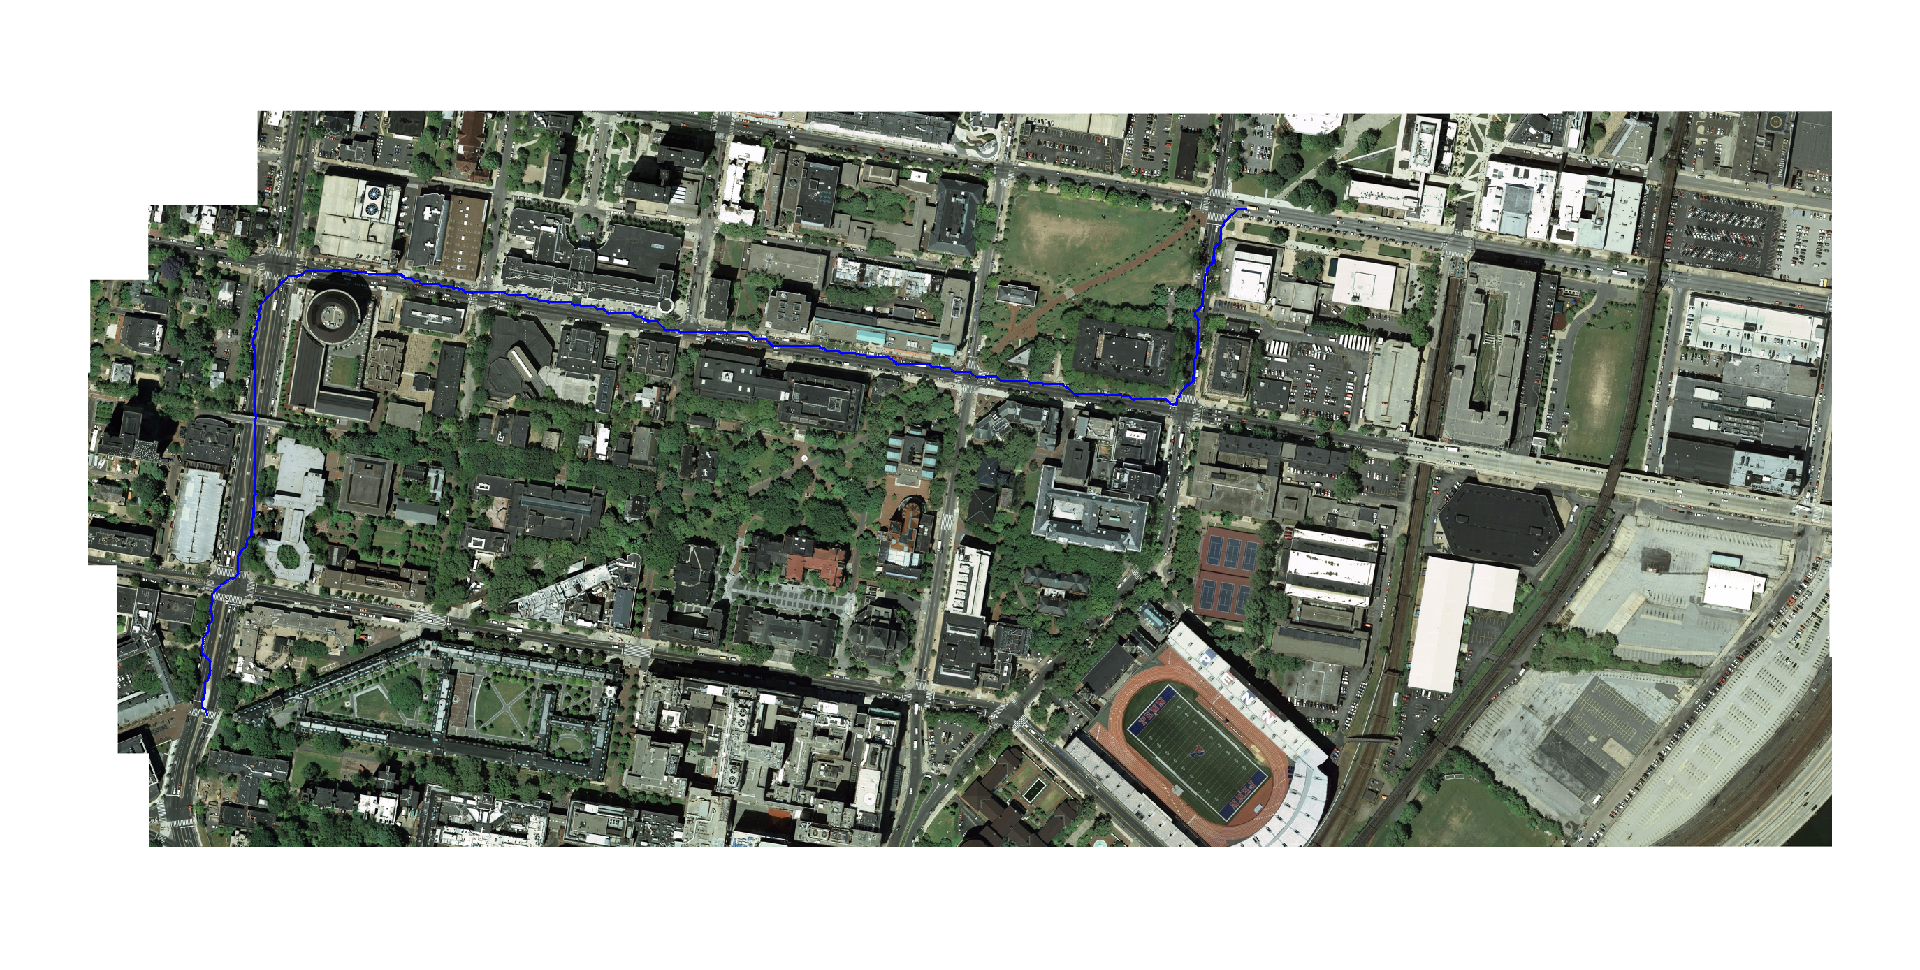
\includegraphics[width=\textwidth]{veh_1}
\caption{Result 1 for the vehicle mode}
\end{figure}

\begin{figure}[thpb]
\centering
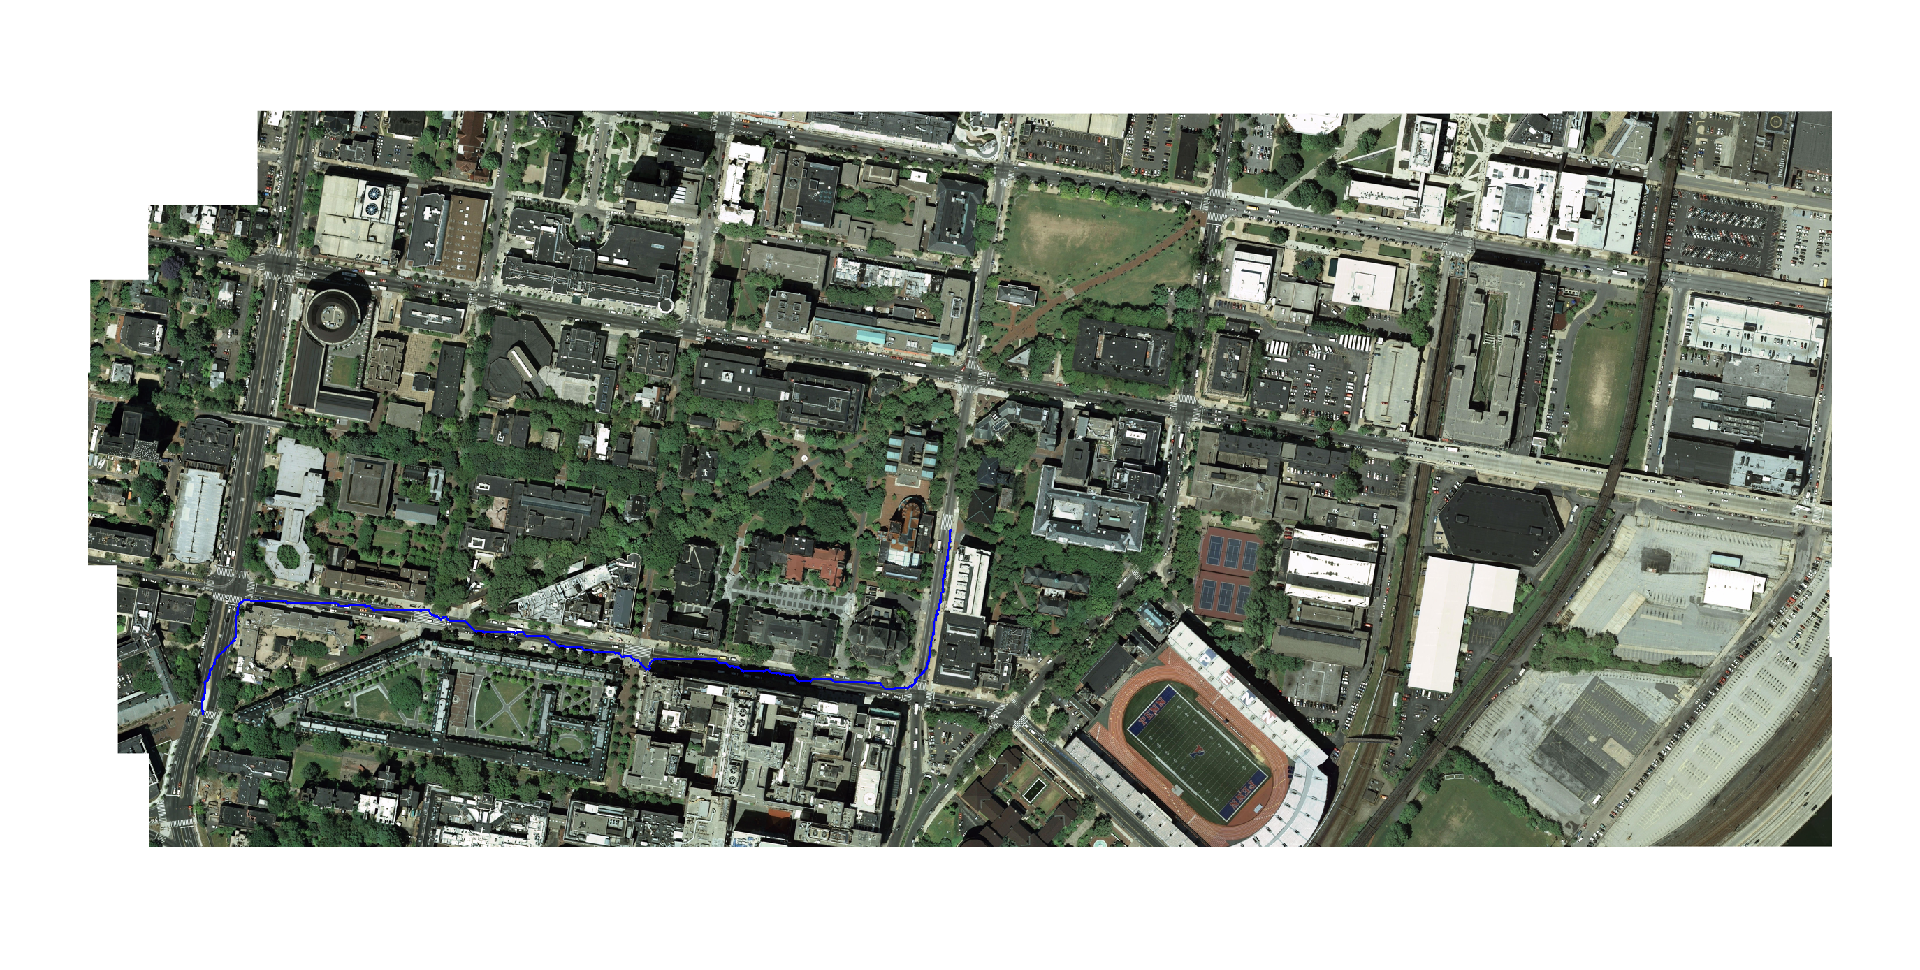
\includegraphics[width=\textwidth]{veh_2}
\caption{Result 2 for the vehicle mode}
\end{figure}

\begin{figure}[thpb]
\centering
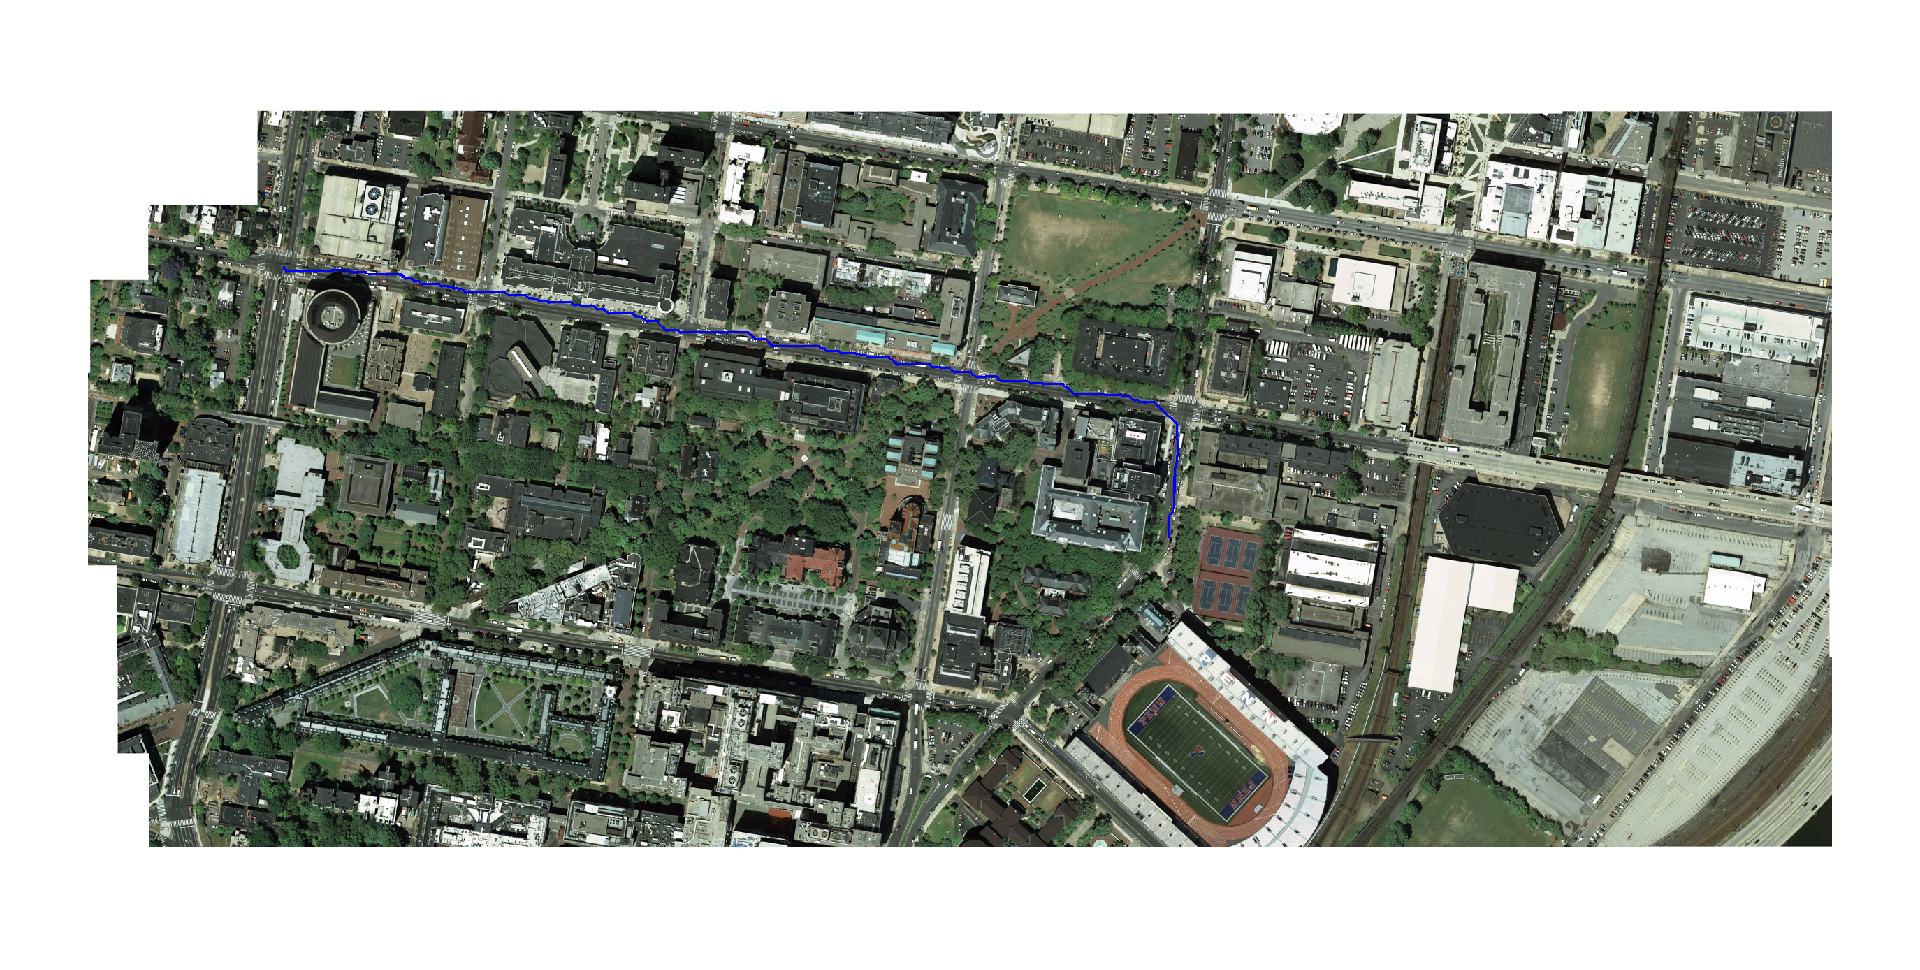
\includegraphics[width=\textwidth]{veh_5}
\caption{Result 3 for the vehicle mode}
\end{figure}

\begin{figure}[thpb]
\centering
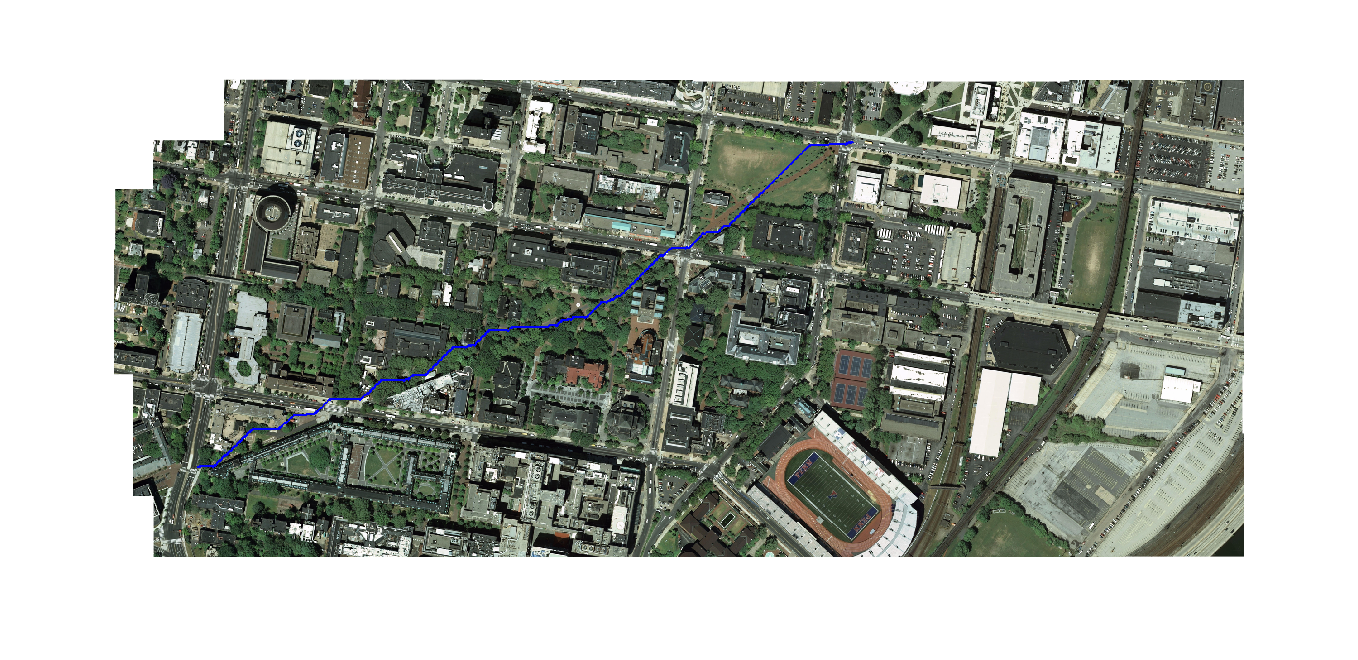
\includegraphics[width=\textwidth]{ped_1}
\caption{Result 1 for the pedestrian mode}
\end{figure}

\begin{figure}[thpb]
\centering
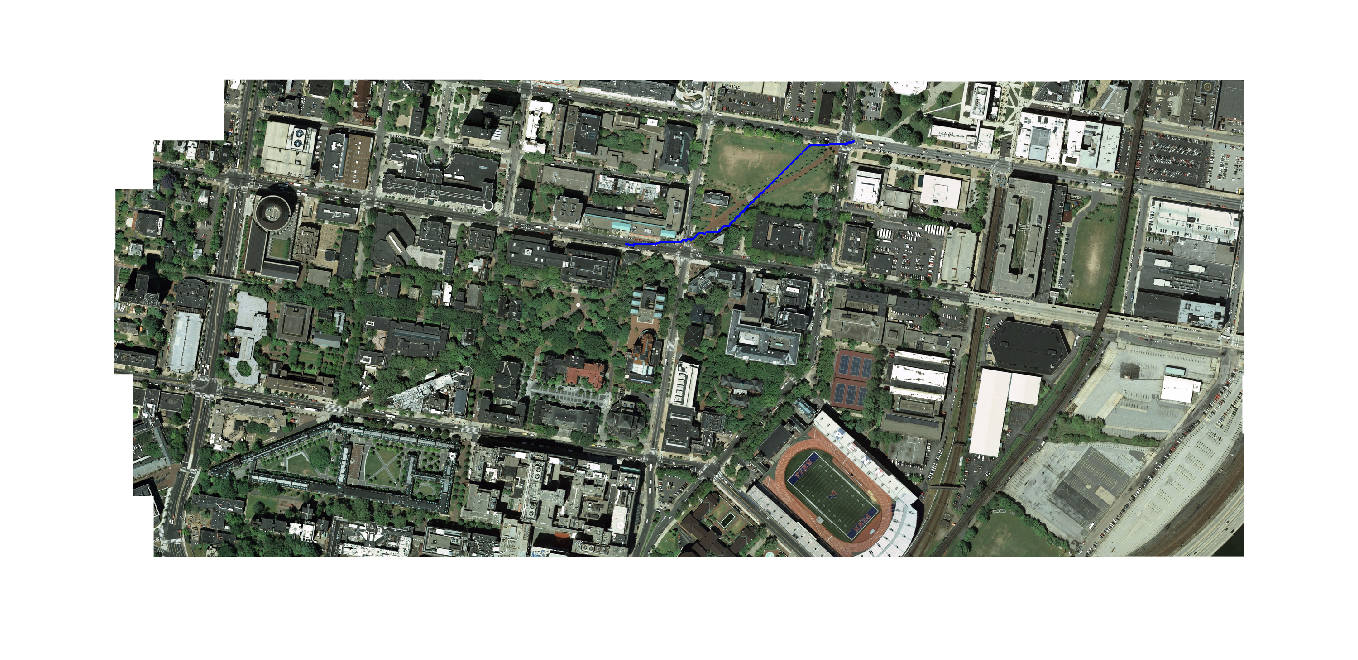
\includegraphics[width=\textwidth]{ped_3}
\caption{Result 2 for the pedestrian mode}
\end{figure}

\begin{figure}[thpb]
\centering
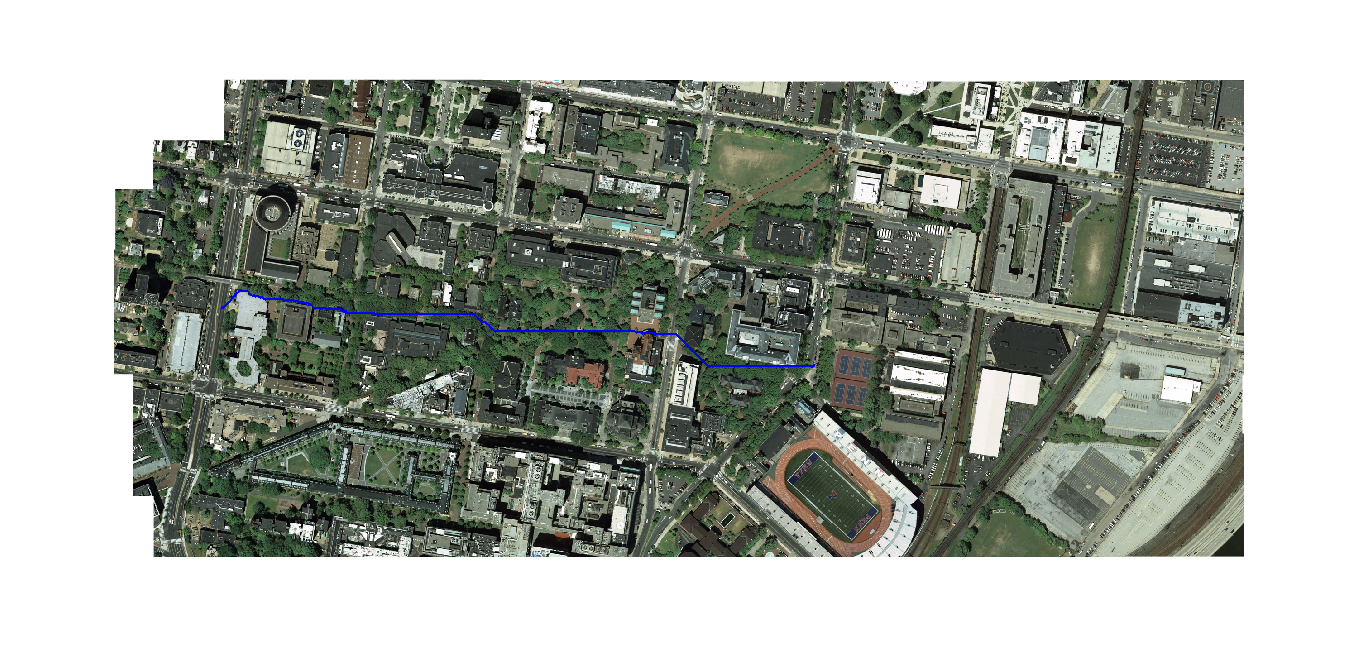
\includegraphics[width=\textwidth]{ped_5}
\caption{Result 3 for the pedestrian mode}
\end{figure}
 




%\bibliographystyle{unsrt}%Used BibTeX style is unsrt
%\bibliography{sample}

\begin{thebibliography}{99}
\bibitem{c1} Nathan D. Ratliff, David Silver, J. Andrew Bagnell. Learning to Search: Functional Gradient Techniques for Imitation Learning
\bibitem{c2} R.-E. Fan, K.-W. Chang, C.-J. Hsieh, X.-R. Wang, and C.-J. Lin. LIBLINEAR: A library for large linear classification Journal of Machine Learning Research 9(2008), 1871-1874.
\end{thebibliography}

\end{document}
